\documentclass[12pt,notitlepage]{article}

% Overleaf project:
% https://www.overleaf.com/project/5fdb880ef955c3369964d601

% View-only link:
% https://www.overleaf.com/read/hkybwqtbtvjb

\usepackage{amsmath, amsfonts, amssymb}
\usepackage[svgnames]{xcolor}
\usepackage{datetime2}
\usepackage[
	colorlinks=true, 
	citecolor={DarkRed}, urlcolor={DarkBlue}, linkcolor={DarkBlue},
]{hyperref}


% 
\usepackage[version=4]{mhchem}

\usepackage{fullpage}

% Paragraph spacing
\usepackage{parskip}

\usepackage{xspace}

\usepackage{graphicx}
\graphicspath{{../code/20201231_SymBio_All/}{../images/}}
\DeclareGraphicsExtensions{.pdf,.eps,.png}

% https://tex.stackexchange.com/questions/202046/width-of-the-caption-of-a-figure
% https://tex.stackexchange.com/questions/29039/how-to-limit-the-figure-caption-width
\usepackage[margin=20px]{caption}

% https://tex.stackexchange.com/questions/20792/how-to-superimpose-latex-on-a-picture
\usepackage[percent]{overpic}

%\usepackage{epstopdf}

% Tables (the order matters here)
\usepackage{makecell}
\usepackage{booktabs}
\usepackage{arydshln}

% https://tex.stackexchange.com/questions/109467/footnote-in-tabular-environment
\usepackage{footnote}
\makesavenoteenv{tabular}
\makesavenoteenv{table}

% https://tex.stackexchange.com/questions/10130/use-the-values-of-title-author-and-date-on-a-custom-title-page
\usepackage{authoraftertitle}

% https://en.wikibooks.org/wiki/LaTeX/Footnotes_and_Margin_Notes#Margin_Notes
\usepackage{marginnote}

% For editing purposes:
%\usepackage[margin=10pt]{geometry}

% https://latex.org/forum/viewtopic.php?t=10456
\usepackage{titlesec}
\titleformat{\subsubsection}[runin]% runin puts it in the same paragraph
{\normalfont\bfseries}% formatting commands to apply to the whole heading
{\thesubsubsection}% the label and number
{}% space between label/number and subsection title
{}% formatting commands applied just to subsection title
[.]% punctuation or other commands following subsection title


\newcommand{\TODO}[1]{\textrm{\color{red}TODO: #1}}

% https://bitbucket.org/goodnightmath/covariance/src/master/tex/main.tex

%%%%%%%%%%%%%%%%%%%%%%%%%%%%%%%%%%%%%%%%%%%%%%%%%%%%%%%%%%%%%%%%%%%%%%%%%%%%%%%
% http://tex.stackexchange.com/a/106577/44073
\usepackage{ifthen}
\newcounter{todoindex}\setcounter{todoindex}{0}
\newcommand\ADDTODO[1]{%
	\addtocounter{todoindex}{1}%
	\expandafter\gdef\csname todo\roman{todoindex}\endcsname{#1}%
	%\expandafter\csname todolabel\roman{todoindex}\endcsname
	\label{todolabel\roman{todoindex}}
}
\renewcommand\TODO[1]{%
	{%
		\ADDTODO{#1}%
		{\textrm{\color{red}TODO(\arabic{todoindex}): #1}}%
	}%
}
\newcommand\CHECK[1]{%
	\ADDTODO{CHECK CLAIM: {#1}}%
	{\color{toverify}#1}%
	\smash{\marginnote{\text{\color{red}*}}}%
}
\newcounter{indextodo}
\newcommand{\SHOWTODOS}{%
	\setcounter{indextodo}{0}%
	\begin{enumerate}
	\item[{\color{red} TODOs:}]
	\whiledo{\value{indextodo} < \value{todoindex}}{%
		\addtocounter{indextodo}{1}%
		\item[\color{red}\arabic{indextodo}.]
		p.\pageref{todolabel\roman{indextodo}}.
		%
		\csname todo\roman{indextodo}\endcsname
	}%
	\end{enumerate}
}
%%%%%%%%%%%%%%%%%%%%%%%%%%%%%%%%%%%%%%%%%%%%%%%%%%%%%%%%%%%%%%%%%%%%%%%%%%%%%%%



\renewcommand{\d}{\mathrm{d}}

\newcommand{\NOT}{\ensuremath{\mathop{\mathsf{not}}}\xspace}
\newcommand{\AND}{\ensuremath{\mathop{\mathsf{and}}}\xspace}
\newcommand{\OR}{\ensuremath{\mathop{\mathsf{or}}}\xspace}
\newcommand{\XOR}{\ensuremath{\mathop{\mathsf{xor}}}\xspace}

\newcommand{\TEXT}[1]{\quad\text{#1}\quad}
\newcommand{\with}{\text{$\,{:}\,$}}

\newcommand{\cbra}[1]{{\ensuremath{\color{gray}{#1}}}}
\newcommand{\signal}[1]{{{\cbra{\langle}\ce{#1}\cbra{\rangle}}}}
\newcommand{\protein}[1]{{{\cbra{(}\ce{#1}\cbra{)}}}}
\newcommand{\promoter}[1]{{{\cbra{[}\ce{#1}\cbra{]}}}}

% https://tex.stackexchange.com/questions/543953/arrow-with-blunted-end-head-in-math-mode
\newcommand{\act}{\ {\ensuremath{\mathbin{\to}}}\ }
\newcommand{\rep}{\ {\ensuremath{\mathrel{\raisebox{-.3ex}{\rotatebox{90}{\scalebox{1}[1.2]{$\bot$}}}}}}\ }

\def\[#1\]{\begin{align}#1\end{align}}

% https://tex.stackexchange.com/questions/114113/how-to-label-text-with-equation-number
\newcommand{\eqnum}{\leavevmode\hfill\refstepcounter{equation}\textup{{(\theequation)}}}

\newcommand{\starlink}[1]{\textsuperscript{\makebox[0pt]{\href{#1}{\color{white}$\star$}}}}

\newcommand{\hh}[1]{{\color{Purple}#1}}
\newcommand{\ra}[1]{{\color{Blue}#1}}


\title{ibiocomp project}
\author{RA \& HH}
\date{\today}
\newcommand{\linktodoc}{http://bit.ly/15sticks}


\begin{document}

\maketitle

% \ra{LOCKED 'COS WORKING WITH ANOTHER COPY (WRITE EMAIL IF NEEDED)}


%%%%%%%%%%%%%%%%%%%%%%%%%%%%%%%%%%%%%%%%%%
\section{Introduction}
%%%%%%%%%%%%%%%%%%%%%%%%%%%%%%%%%%%%%%%%%%

\subsection{The game of 15 sticks}

We design genetic circuits
that play the following game:
%
\begin{quote}
	Two players start with 15 sticks
	and alternatingly 
	take 1, 2 or 3 sticks.
	\\
	The last player to take a stick loses.
\end{quote}

Because a player can complement
the number of sticks taken by the opponent,
there is a deterministic winning strategy
of the first-mover
as shown in Table \ref{t:logical-playera}.
%
%
We implement this strategy for both players.


\subsection{General design} \label{s:general}

We encode in binary 
the number of sticks left as
\[
    \label{e:s0123}
    %
    \text{number of sticks left} = \ce{8 s_3 + 4 s_2 + 2 s_1 + s_0}
    .
\]
%
%
By the 4-periodicity of the winning strategy,
only the two lowest bits \ce{s_1}/\ce{s_0}
matter to the player.
%
%
The response of a player is a number 1, 2, or 3,
which we encode in binary as
\[
    \label{e:r01}
    %
    \text{number of sticks taken by a player} = \ce{2 r_1 + r_0}
    .
\]
%
The bits in \eqref{e:s0123}--\eqref{e:r01}
are transmitted 
between compute units
by 
intercellular signaling molecules,
cf.~\S\ref{ss:experiment}.
%
Although our players are essentially identical,
we model them separately and with one difference:
Player A (B) becomes active when 
the extracellular signal \ce{w_A} (\ce{w_B}) is supplied.

%

The \emph{subtractor} module
keeps track of the number of sticks left \eqref{e:s0123}.
To appreciate the key design issue, suppose
we manually transmit the response \ce{r_1 r_0 = 01}
of a player
into the medium of the subtractor.
It should compute the new number of the sticks,
yet, it has to do so once
and not keep subtracting the value \ce{r_1 r_0}
that is still present.
One solution is single-use subtractors
but then the result of each computation
has to be imparted to an unused subtractor.
Barring excessive manual intervention,
a feasible design
seems to require some separation of
reading/storing the current state,
computing the new state and communicating it
--
temporally or spatially.
%
% For our purposes this may include
% modest parallelism in intercellular signaling
% (but not frequency encoding).
\marginnote{\ra{removed sentence}}
%
%
We propose 
a subtractor composed of two parts A and B,
and
a workflow 
%of Phase A, Interphase, Phase B, Interphase, etc.,
as shown in Table \ref{t:workflow}.
%
%
%
Thus,
in Phase A characterized by the supply of 
the master signal \ce{w_A},
Subtractor A
emits the current state \ce{s},
Player A responds with \ce{r},
while
Subtractor B
reads \ce{s}/\ce{r}
and
computes the new state % \ce{s} 
{silently}
and remembers the result
in order to emit it in the subsequent Phase B.
%
\ra{
We use the symbols \ce{d_3}/\ce{d_2}/\ce{d_1}/\ce{d_0}
for this internal state.
}
%
The medium is cleared, before
Phase B is initiated by
supplying the master signal \ce{w_B}.
%
%
In short,
we require
a gated memory module and a delayed response,
cf.~\S\ref{ss:sub}.
%
%

%

Refinements could include
a)
dealing with
a player who attempts to take more sticks than \eqref{e:s0123};
b)
dedicated sensor cells 
that report on signaling molecules 
in order to 
monitor the state of the game.

%

%%% TABLE %%%


\begin{table}[hpbt]
	\centering 
	
	% Table made by this script:
	% https://deepnote.com/project/998c51eb-bb3f-4a0f-88e3-c8b50d4d678a#%2Ft_phases.ipynb
	\begin{tabular}{llll}
	\toprule
	{} &                                Phase A &               Interphase I &                                Phase B \\
	\midrule
	Experimenter &                        supply \ce{w_A} &  \makecell{clear medium} &                        supply \ce{w_B} \\
	Player A     &                in: \ce{s}, out: \ce{r} &                       -- &                                     -- \\
	Subtractor A &                        out: new \ce{s} &                       -- &  in: \ce{s}/\ce{r}; \makecell{compute} \\
	Subtractor B &  in: \ce{s}/\ce{r}; \makecell{compute} &                       -- &                        out: new \ce{s} \\
	Player B     &                                     -- &                       -- &                in: \ce{s}, out: \ce{r} \\
	\bottomrule
	\end{tabular}
	
	\caption{%
		Workflow:
		Phases I/A/I/B
		alternate
		until the game is over.
	}
	
	\label{t:workflow}
\end{table}





\subsection{Conventions}


\ra{
%
As shown in Table \ref{t:signals},
we encode \ce{w_A} by L-arabinose,
\ce{w_B} by IPTG, etc.
%
Our convention is \ce{w_A = 1}
if 
the corresponding messenger molecule L-arabinose 
is present in the medium or in the cell 
in sufficiently high quantity,
and \ce{w_A = 0} otherwise.
%
We write \ce{\#w_A} for
the \emph{number} of L-arabinose molecules 
in the numerical simulations.
%
We may abbreviate
{3OC6}{-}HSL by {3OC6}.
%
Where suitable,
we indicate the semantics of an element thus:
\signal{signal},
\protein{protein} -- often a transcription factor,
and
\promoter{promoter};
%
this is consistent with 
the symbols that we employ in
the SimBiology schemes.
%
We may write \signal{w_A} to mean 
``the signal molecule that encodes \ce{w_A}'',
i.e.~L-arabinose.
%
Ditto for the other signals.
}
%
%
%
\ra{
Abbreviations:
RBS = ribosome binding site.
}


\subsection{Logic circuits}


\subsubsection*{The players} \label{ss:players}

Both players
follow the same deterministic strategy,
which is a winning strategy for the first-mover.
%
They are identical except
that player A responds when \ce{w_A} is present
and player B responds upon \ce{w_B}.
%
The logic is shown in Table \ref{t:logical-playera}.

%%% TABLE %%%
% Generated in part using

% https://github.com/numpde/ibiocomp/blob/main/code/20201229_LogicalTables/PlayerA.py

% and
	
% https://crcit.net/c/205b0db18f954c4585b3f87d69fced6c
% https://crcit.net/c/84159c89986c4330978603aeace14aa1

% RA, 2020-12-30
	
\begin{table}[hpbt]
	\centering

	\begin{minipage}{0.3\linewidth}
		\centering
				
		Winning strategy:
		
		{\ }
		
		\begin{tabular}{cccc|c}
		\multicolumn{4}{c|}{Sticks left} & Take \\
		\hline
		15 & 11 & 7 & 3 & 2 \\
		14 & 10 & 6 & 2 & 1 \\	
		13 & 9  & 5 & 1 & 1 \\	
		12 & 8  & 4 &   & 3 \\	
		\end{tabular}
	\end{minipage}
	%
	\qquad
	%
	\begin{minipage}{0.25\linewidth}
		\centering
		\begin{tabular}{ccc|cc}
		\cee{w_A} &  \cee{s_1} &  \cee{s_0} &  \cee{r_1} &  \cee{r_0} \\
		\hline
		  0 &   0 &   0 &   0 &   0 \\
		  0 &   0 &   1 &   0 &   0 \\
		  0 &   1 &   0 &   0 &   0 \\
		  0 &   1 &   1 &   0 &   0 \\
		  1 &   0 &   0 &   1 &   1 \\
		  1 &   0 &   1 &   0 &   1 \\
		  1 &   1 &   0 &   0 &   1 \\
		  1 &   1 &   1 &   1 &   0 \\
		\end{tabular}
	\end{minipage}
	%
	\qquad
	%
	\begin{minipage}{0.3\textwidth}
		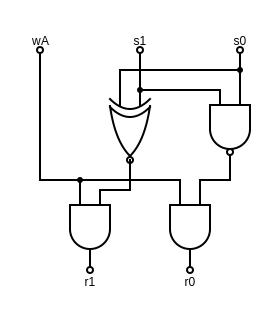
\includegraphics[width=\linewidth]{circuits/Logical-PlayerA}
	\end{minipage}
	
	\caption{%
		Logical circuit for {Player A}.
		%
		The input is a
		wake-up signal \cee{w_A}
		and the bits
		\cee{s_1}/\cee{s_0}
		of the current number of sticks
		(\cee{8 s_3 + 4 s_2 + 2 s_1 + s_0}).
		%
		The output is
		the number of sticks that 
		the player chooses to take,
		encoded as \cee{2 r_1 + r_0}.
		%
		Note that the output is cut off
		when \cee{w_A} is absent.
		%
		%
		The circuit for {Player B}
		is identical except
		that it is controlled up by \cee{w_B}.
	}
	
	\label{t:logical-playera}
\end{table}



\subsubsection*{Subtractor} \label{ss:sub}

\ra{
In Phase A,
Subtractor B 
senses the current number of sticks \eqref{e:s0123},
emitted by Subtractor A,
and 
the response \eqref{e:r01} from Player A,
and
computes the difference \ce{d}.
%
It has four compute units Bit~0 to Bit~3
that are also
spatially separated (cf.~\S\ref{ss:experiment}). 
%
The subtraction proceeds from Bit~0 to Bit~3
(cf.~Table~\ref{t:substeps}).
%
Bit~0 senses the current \ce{s_0}/\ce{r_0}
and computes \ce{d_0} (silently)
and the carry flag \ce{c_1} (emitted immediately).
%
The carry flag is passed on to Bit~1.
%
Bit~1 subtracts \ce{r_1} and \ce{c_1} from \ce{s_1}. 
%
The resulting carry flag \ce{c_2} 
is passed on to Bit~2, 
which subtracts \ce{c_2} from \ce{s_2}.
%
Then Bit~3 subtracts the resulting carry flag
\ce{c_3} from \ce{s_3}.
%
Importantly,
each of
Bit 0/2/3,
is in fact a ``half-subtractor'' with 2 inputs,
whilst
Bit~1 is a ``full subtractor'' with 3 inputs.
}
%
\ra{
See
Table~\ref{t:subtractor1}
for the truth table
of the subtraction.
%
Fig.~\ref{f:logical-subtractor01}
shows a reference logic circuit 
for Bit~0 and Bit~1
that illustrates the principle of delayed response.
}

%%% TABLE %%%
% Generated in part using
% https://github.com/numpde/ibiocomp/blob/main/code/20201229_LogicalTables/Subtractor.py

% RA, 2020-12-30

\begin{table}[hpbt]
\centering

\begin{minipage}{0.2\linewidth}
	\centering
			
	Half-subtractor:
	
	{\ }
	
	\begin{tabular}{cc|cc}
		\ce{s_3} &  \ce{c_3} &  \ce{d_3} &  -- \\
		\hdashline
		\ce{s_2} &  \ce{c_2} &  \ce{d_2} &  \ce{c_3} \\
		\hdashline
		\ce{s_0} &  \ce{r_0} &  \ce{d_0} &  \ce{c_1} \\
		\hline
         0 &          0 &          0 &          0 \\
         0 &          1 &          1 &          1 \\
         1 &          0 &          1 &          0 \\
         1 &          1 &          0 &          0 \\
	\end{tabular}
\end{minipage}
%
\quad
%
\begin{minipage}{0.3\linewidth}
	\centering
			
%		Full subtractor:
%		
%		{\ }
	
	\begin{tabular}{ccc|cc}
		\ce{s_1} &  \ce{r_1} &  \ce{c_1} &  \ce{d_1} &  \ce{c_2} \\
		\hline
         0 &          0 &          0 &          0 &          0 \\
         0 &          0 &          1 &          1 &          1 \\
         0 &          1 &          0 &          1 &          1 \\
         0 &          1 &          1 &          0 &          1 \\
         1 &          0 &          0 &          1 &          0 \\
         1 &          0 &          1 &          0 &          0 \\
         1 &          1 &          0 &          0 &          0 \\
         1 &          1 &          1 &          1 &          1 \\
	\end{tabular}
\end{minipage}
%
\quad
%
\begin{minipage}{0.3\linewidth}
	\begin{align*}
		\ce{& & 8 s_3 + 4 s_2 + 2 s_1 + s_0 &}
		\\
		- \ce{& & 2 r_1 + r_0 &}
		\\
		= \ce{& & 8 d_3 + 4 d_2 + 2 d_1 + d_0 &}
	\end{align*}
\end{minipage}

\caption{%
	The subtractor computes
	\ce{d = s - r} (mod 16).
	%
	Since \ce{r} only has 
	the two lowest bits, 
	a half-subtractor
	is sufficient for
	the bits \ce{d_0}/\ce{d_2}/\ce{d_3}
	and the carry flags \ce{c_1}/\ce{c_3},
	and
	only \ce{d_1}/\ce{c_2}
	require the full subtractor.
	%
	We have $\ce{d_0} = (\ce{s_0} \XOR \ce{r_0})$;
	$\ce{c_1} = \NOT (\ce{s_0} \geq \ce{r_0})$;
	$\ce{d_1} = ((\ce{s_1} + \ce{r_1} + \ce{c_1}) \mathbin{\mathrm{mod}} 2)$;
	$\ce{c_2} = \NOT (\ce{s_1} \geq \ce{r_1} \geq \ce{c_1})$.
	%
	See Fig.~\ref{f:logical-subtractor01}
	for a logic circuit of
	the subtractor.
}
\label{t:subtractor1}
\end{table}









\subsection{Experimental design} \label{ss:experiment}

We distinguish
\emph{extracellular} chemical signals 
that are supplied by the experimenter
(the master signals \ce{w_A}/\ce{w_B})
and
\emph{intercellular} signals
that are produced and sensed by cells.
%
%
%
For an experiment in a single test tube 
we need
orthogonal intercellular channels:
\emph{three} for \eqref{e:s0123}
($s_3$ has no downstream),
\emph{two} for \eqref{e:r01},
and
\emph{three} for the carry flags
(see \S\ref{ss:sub}).
%
One channel could be spared 
at the expense
of a more involved computation of 
the last useful carry flag $c_3$.
%
Thus we need \emph{eight} orthogonal intercellular channels,
cf.~Table \ref{t:substeps}.
%
In \cite{DuETAL2020},
ten de novo intercellular signaling pathways
were designed
and
four known QS pathways
were optimized,
however,
only \emph{eight} worked well orthogonally
on the sensor level 
and 
seven on the promoter level
\cite[\href{https://www.nature.com/articles/s41467-020-17993-w/figures/3}{Fig.~3c/g}]{DuETAL2020}.
%
We have tried to assign the signals
to further minimize crosstalk,
in particular 
avoiding LuxR and RpaR in one cell
as warned in \cite[p.6]{DuETAL2020}.
%
The signals are listed in
Table~\ref{t:signals}.
%
%
%

%%% TABLE %%%

\begin{table}[hpbt]
\centering

\begin{tabular}{clrr}
	Bit
	&
	\signal{signal}, \protein{txn factor}, \promoter{promoter}
	&
	Primary reference
	&
	Details

	\\
	
	\hline
	
	\ce{w_A}
	& 
	$
		\href{https://pubchem.ncbi.nlm.nih.gov/compound/L-Arabinose}{\signal{Ara}}
		\act
		\protein{AraC^*}
		\act
		\promoter{BAD}
	$
	&
	\cite[SM, VII.M]{NielsenETAL2016}
	& 
	\S\ref{ss:wAB}/p.\pageref{ss:wAB}
	
	\\
	
	\ce{w_B}
	&
	$
		 \href{https://pubchem.ncbi.nlm.nih.gov/compound/656894}{\signal{IPTG}}
		 \rep
		 \protein{LacI}
		 \rep
		 \promoter{Tac}
	$
	&
	\cite[SM, VII.M]{NielsenETAL2016}
	&
	\S\ref{ss:wAB}/p.\pageref{ss:wAB}
	
	\\
	
	\ce{r_0}
	&
	$
		 \href{https://pubchem.ncbi.nlm.nih.gov/compound/119133}{\signal{{3OC6}{-}{HSL}}}
		 \act
		 \protein{LuxR}
		 \act
		 \promoter{Lux}
	$
	&
	\cite[\href{https://www.embopress.org/doi/full/10.15252/msb.20156590}{p.1}]{Grant2016}
	&
	\S\ref{ss:3OC6}/p.\pageref{ss:3OC6}
	
	\\
	
	\ce{r_1}
	&
	$
		\href{https://pubchem.ncbi.nlm.nih.gov/compound/71627311}{\signal{IV{-}HSL}}
		\rep
		\protein{BjaR}
		\rep
		\promoter{Bja}
	$
	&
	\cite[\href{https://www.nature.com/articles/s41467-020-17993-w\#Sec23}{SM}:p.2]{DuETAL2020}
	&
	\S\ref{ss:IV}/p.\pageref{ss:IV}

	\\
	
	\ce{s_0}
	&
		$
		\href{https://pubchem.ncbi.nlm.nih.gov/compound/2_4-Diacetylphloroglucinol}{\signal{DAPG}}
		\rep
		\protein{PhlF}
		\rep
		\promoter{PhlF}
	$
	&
	\cite[\href{https://www.nature.com/articles/s41467-020-17993-w\#Sec23}{p.2}]{DuETAL2020}
	
	&
	\S\ref{ss:DAPG}/p.\pageref{ss:DAPG}
	
	\\
	
	\ce{c_1}
	&
	$
		\href{https://pubchem.ncbi.nlm.nih.gov/compound/338}{\signal{Sal}}
		\act
		\protein{NahR}
		\act
		\promoter{Sal}
	$
	&
	\cite[\href{https://www.nature.com/articles/s41467-020-17993-w\#Sec23}{SM}:p.2]{DuETAL2020}
	
	&
	\S\ref{ss:Sal}/p.\pageref{ss:Sal}
   
	\\
	
	\ce{s_1}
	&
	$
		\href{https://pubchem.ncbi.nlm.nih.gov/compound/N-_4-Coumaroyl_-L-homoserine-lactone}{\signal{pC{-}HSL}}
		\act
		\protein{RpaR}
		\act
		\promoter{Rpa}
	$
	&
	\cite[\href{https://www.nature.com/articles/s41467-020-17993-w\#Sec23}{p.2}]{DuETAL2020}
	&
	\S\ref{ss:pC}/p.\pageref{ss:pC}
	
	\\
	
	\ce{c_2}
	&
	$
		\href{https://pubchem.ncbi.nlm.nih.gov/compound/13265877}{\signal{MMF}}
		\rep
		\protein{MmfR}
		\rep
		\promoter{Mmf}
	$
	&
	\cite[\href{https://www.nature.com/articles/s41467-020-17993-w\#Sec23}{SM}:p.2]{DuETAL2020}
	&
	\S\ref{ss:MMF}/p.\pageref{ss:MMF}
	
	\\
	
	\ce{s_2}
	&
	$
		\href{http://www.chemspider.com/Chemical-Structure.2497481.html}{\signal{{3OC12}{-}HSL}}
		\act
		\protein{LasR}
		\act
		\promoter{Las^*}
	$ 
	&
	\cite[\href{https://www.nature.com/articles/s41467-020-17993-w\#Sec23}{SM}:p.3]{DuETAL2020}
	&
	\S\ref{ss:3OC12}/p.\pageref{ss:3OC12}
	
	\\
	
	\ce{c_3}
	&
	$
        \href{https://pubchem.ncbi.nlm.nih.gov/compound/932}{\signal{NG}}
		\act
		\protein{FdeR}
		\act
		\promoter{FdeA}
	$
	\hh{act}
	&
	\cite[\href{https://www.nature.com/articles/s41467-020-17993-w\#Sec23}{SM}:p.3]{DuETAL2020}
	&
	\S\ref{ss:NG}/p.\pageref{ss:NG}
\end{tabular}

\caption{%
	Extra-/intercellular \signal{signals}
	with downstream 
	\protein{factors}
	and
	\promoter{promoters}.
}
%
\label{t:signals}

\TODO{what is MMF?}

\hh{Links to pubchem. Please check}
\end{table}



%

\ra{
To facilitate debugging
we partition the workflow
with spatial compartments
that require manual transmission of 
the medium.
%
%
Unfortunately, this does not automatically reduce
the number of intercellular channels needed.
}


\TODO{what species are we working with}


\TODO{experimental protocol:}
%
In phase A.
%
Add \ce{w_A} everywhere.
%
Then:
%
\begin{enumerate}
\item 
    Admix the medium of Bit~0 and Bit~1 
    (containing the signals \ce{s_0} and \ce{s_1})
    to Player~A,
    wait for Player~A to respond
    (with \ce{r_0}/\ce{r_1}).
    
\item
    Admix the medium of Player~A
    (with \ce{r_0}/\ce{r_1}/\ce{s_0}/\ce{s_1})
    to Bit~0, wait for response
    (with \ce{c_1}).
    
\item
    Admix the media of Player~A and Bit~0
    (with \ce{r_0}/\ce{r_1}/\ce{s_0}/\ce{s_1}/\ce{c_1})
    to Bit~1, wait for response
    (with \ce{c_2}). 
    
\item
    
\item
    Admix the medium from Bit~3 to Bit~4.
    
\end{enumerate}




\begin{table}[hpbt]
    \centering
    %
    % Table made with
    % https://deepnote.com/project/998c51eb-bb3f-4a0f-88e3-c8b50d4d678a#%2Ft_phases.ipynb
    %
    \begin{tabular}{l||cc|ccc|ccc|ccc|cc}
    {} &      \ce{r_0} &      \ce{r_1} &    \ce{s_0} &      \ce{d_0} &      \ce{c_1} &      \ce{s_1} & \ce{d_1} &      \ce{c_2} &    \ce{s_2} &      \ce{d_2} &      \ce{c_3} &    \ce{s_3} &      \ce{d_3} \\ 
    \hline
    1 &  $\downarrow$ &  $\downarrow$ &  $\uparrow$ &               &               &    $\uparrow$ &          &               &             &               &               &             &               \\ 
    \hline
    2 &    $\uparrow$ &               &  $\uparrow$ &  $\downarrow$ &  $\downarrow$ &               &          &               &             &               &               &             &               \\ 
    \hline
    3 &               &    $\uparrow$ &             &               &    $\uparrow$ &  $\downarrow$ &          &  $\downarrow$ &             &               &               &             &               \\ 
    \hline
    4 &               &               &             &               &               &               &          &    $\uparrow$ &  $\uparrow$ &  $\downarrow$ &  $\downarrow$ &             &               \\ 
    \hline
    5 &               &               &             &               &               &               &          &               &             &               &    $\uparrow$ &  $\uparrow$ &  $\downarrow$ \\ 
    \hline
    \end{tabular}
    %
    %
    \caption{%
        Substeps of each phase A/B.
        Arrows: emit ($\uparrow$) and compute ($\downarrow$).
    }
    \label{t:substeps}
\end{table}


\TODO{mention a microfluids setup?}


\TODO{Specify initial conditions}


\subsection{Cite as}

\MyTitle, \MyAuthor, \MyDate.
\href{\linktodoc}{{\small\texttt{\linktodoc}}}

See this link 
for the Matlab/SymBiology files
and 
for the PDF file with sharp figures.


%%%%%%%%%%%%%%%%%%%%%%%%%%%%%%%%%%%%%%%%%%%
\section{Genetic toolbox} \label{s:genetic}
%%%%%%%%%%%%%%%%%%%%%%%%%%%%%%%%%%%%%%%%%%%


\subsection{Constitutive promoters} \label{ss:const}

\cite{ShimadaETAL2014}

\TODO{const prom}


\subsection{No-questions-asked transcription factors}

\subsubsection*{cI} \label{ss:cI}

\ra{
The optimized and orthogonal variant
$\ce{cI^*} := \ce{cI_{5G6G,P}}$
of the transcription factor $\lambda$~\ce{cI}
from
\cite[\href{https://www.nature.com/articles/ncomms13858/figures/4}{Fig.~4c/d}]{BroedelJaramilloIsalan2016}
requires no cofactors
and
shows 
about 10-fold activation of the promoter
$\promoter{cI^*_+} := \promoter{M,{5G6G}}$
and 
a similar-fold repression of 
$\promoter{cI^*_-} := \promoter{{5G6G}}$.
%
%
To improve the dynamic range of 
$\promoter{cI^*_+} \act \text{mRNA}_1$
we propose 
that
$\promoter{cI^*_-}$ express
an inhibitory RNA that is complementary
to the RBS of $\text{mRNA}_1$.
}




\subsection{3-input gates by Cello} \label{ss:cello}

In
\cite{NielsenETAL2016}
we found these gates
among good performers:
%
\begin{itemize}
\item
    $
    	\ce{r_0} = 
    	\mathop{\mathsf{%
    	\href{https://science.sciencemag.org/content/sci/352/6281/aac7341/F5/graphic-6.large.jpg}{0x0E}%
    	}}
    	(\ce{s_0}, \ce{s_1}, \ce{w_A})
    $,
\item
    $
    	\ce{r_1} =
    	\NOT
    	\mathop{\mathsf{%
    	\href{https://science.sciencemag.org/content/sci/352/6281/aac7341/F5/graphic-5.large.jpg}{0xF6}%
    	}}
    	(\ce{s_0}, \ce{s_1}, \ce{w_A})
    $,
\item
    $
    	\ce{c_2}
    	=
    	\NOT
    	\mathop{\mathsf{%
    	\href{https://science.sciencemag.org/content/sci/352/6281/aac7341/F5/graphic-8.large.jpg}{0x8E}%
    	}}
    	(\ce{c_1}, \ce{r_1}, \ce{s_1})
    	=
       	\mathop{\mathsf{%
    	\href{https://science.sciencemag.org/content/sci/352/6281/aac7341/F5/graphic-5.large.jpg}{0x4D}%
    	}}
       	(\ce{c_1}, \ce{s_1}, \ce{r_1}) 
    $,
    which is
    symmetric in \ce{r_1}/\ce{c_1}.
\end{itemize}
%
%
We did not find the 3-\XOR, see \S\ref{ss:3xor}.
%
%
We used their $\mathsf{0x0E}$ to implement \ce{r_0},
replacing the sensors 
and
replacing the repressor PhlF 
(which clashes with the \ce{s_0} sensor) 
by HlyIIR.
%
The last operation of $\mathsf{0x0E}$
is a ``poor man's \OR gate'';
we let it control the production of \ce{cI^*}
(\S\ref{ss:cI})
that
triggers the synthesis of \signal{r_0}.

%

We noted that \ce{r_1} can reuse 
most of this circuitry.
%
Thus we implemented 
the remainder using ribocomputing
\TODO{explain}.

%

For \ce{c_2}, we took 
the $\NOT \mathsf{0x83}$ construct from \cite{NielsenETAL2016}, 
replacing the sensors.
%
Also, 
we replaced the final 
``$\NOT (\NOT (\cdot) \OR \NOT (\cdot))$''
by
``$(\cdot) \mathbin{\AND} (\cdot)$'',
implemented as a ribo-\AND gate with cross-inhibition,
see \S\ref{ss:xinh}/p.\pageref{ss:xinh}.



\subsection{Intracellular pathways (transducers)}


\subsubsection*{AmtR}

The TetR family member AmtR is 
the central regulator of nitrogen starvation response
in 
the Gram-positive 
\emph{C.~glutamicum}%
\starlink{https://en.wikipedia.org/wiki/Corynebacterium_glutamicum}
\cite{JakobyETAL2000}.
%
This repressor is released
by
the trimeric adenylylated $\mathrm{P_{II}}$-type 
signal-transduction protein GlnK
\cite{BeckersETAL2005, SevvanaETAL2017},
which is present upon
nitrogen starvation. 
%
The AmtR box and the regulon is 
characterized in 
\cite{BeckersETAL2005},
and
several variants are compared 
in \cite{MuhlETAL2009}.
%
%
\TODO{Do we need (to take care of) the GlnK release mechanism?}
%
It seems clear that 
AmtR sits on the DNA as a dimer
\cite{SevvanaETAL2017},
\cite[\S3.4.2]{Schwab2019}.

% Further literature
%\cite{MuhlETAL2009}
%\cite{BuchingerETAL2009}

\subsubsection*{...}

\TODO{continue}


\subsection{Extracellular signaling} \label{ss:wAB}

The two master signals \ce{w_A} and \ce{w_B}
are encoded by L-arabinose and IPTG,
respectively,
and are supplied by the experimenter.
%
%
%
Following \cite[SM, VII.M]{NielsenETAL2016}/\cite{LeeETAL2007}
we posit
a truncated \protein{AraC^*}
that has reduced crosstalk with \signal{IPTG}.
%
%
\ra{
The genetic sequences can be found 
in
\cite[SM, Table~S8]{NielsenETAL2016}
for \protein{Ara^*} and \protein{LacI},
and
in
\cite[SM, Table~S9]{NielsenETAL2016}
for \promoter{BAD} and \promoter{Tac}.
}

% Ref on Ara>AraC>BAD: \cite{LeeETAL2007}
% Ref on IPTG>LacI>Tac: \cite{DykxhoornStpierreLinn1996}



\subsection{Intercellular pathways}

\TODO{references to \cite{DuETAL2020}}

\TODO{comment on toxicity, see SM of Du}

\TODO{WHAT ABOUT THE SENDERS?}



	
\subsubsection*{3OC6} \label{ss:3OC6}
 
The transcription activator \protein{LuxR}
occurs in Gram-negative bacteria
such as 
\emph{V.~fischeri}%
\starlink{https://en.wikipedia.org/wiki/Aliivibrio_fischeri}%
.
%
The bacterium is permeable to the (auto)inducer
3‐oxo‐C6‐homoserine lactone (3OC6-HSL) .
%
The inducer 
\hh{belongs to \ra{the} acyl homoserine lactone (AHL) \ra{family?}
that \ra{is} commonly used
\ra{by whom? ref?}
in quorum sensing
\ra{perhaps better to say which ones are in one place (at the beginning of this subsection) with an appropriate ref}
}. 

It binds to the N-terminal of \protein{LuxR},
which otherwise inhibits its
functional C-terminal \cite{StevensDolanGreenberg1994}.
%
%
The purified C-terminal binds 
upstream of the \emph{lux} box 
(which is centered at $-42.5$bp \cite{EglandGreenberg1999});
however, 
together with the RNA Pol,
it protects the \emph{lux} box and the \emph{lux} operon
promoter
\cite{StevensDolanGreenberg1994}.
%
\TODO{finish}


\subsubsection*{IV} \label{ss:IV}

\TODO{describe}

\subsubsection*{DAPG} \label{ss:DAPG}

\TODO{describe}

\subsubsection*{Sal} \label{ss:Sal}

According to 
\cite{SchellWender1986, HuangSchell1991},
the transcription activator \protein{NahR}
binds to the recognition site of \promoter{Sal} at
$-83$ to $-45$
without the inducer \cite[p.10837]{HuangSchell1991}.
%
%
%
In \cite{SchellBrownRaju1990},
it was suggested 
that the active configuration of \protein{NahR} is a tetramer,
while \cite{ParkLimShin2005}
reported that 
there could be three different complexes
%
$\protein{NahR} \with \promoter{Sal}$.

\TODO{make coherent}

\hh{
Nevertheless, the configuration changes 
then promotes the RNA polymerase binding near $-35$ (upstream of \promoter{Sal})\cite{HuangSchell1991}.
%
%
The inducer
(here \signal{Sal}) can induce the conformation change of \protein{NahR},
and activates the promoter \promoter{Sal}.
}

%
%
Following \cite{Peking2013},
we suppose
that 
$4 \times \protein{NahR}$ bind to the DNA,
and
transcription starts
once a $\signal{Sal}$
binds to each \protein{NahR}.
%
For the sensors we assume an abundance
of \protein{NahR},
hence the inactive form of the promoter
is $\protein{NahR}_4 \with \promoter{Sal}$.
%
%
\TODO{finish}


\subsubsection*{pC} \label{ss:pC}

\hh{
The p-coumaroyl-HSL/RpaR system 
(pC-HSL)
works similarly to AHL/LuxR system, but the pC-HSL is composed of p-coumaric acid rather than fatty acids in AHL.
%
As pC-HSLs come from an anoxygenic phototrophic soil bacterium strain, 
the luxIR-type pair, rpaI and rpaR shows good orthogonality to many
QS signals in use \cite{SchaeferETAL2008}.
}

\ra{
The \emph{R.~palustris}%
\starlink{https://en.wikipedia.org/wiki/Rhodopseudomonas_palustris}
%
transcriptional regulator
\protein{RpaR},
when purified,
binds an inverted repeat element 
centered at $-48.5$bp
of its promoter
\cite{HirakawaETAL2011}.
%
%
Transcription depends on 
the inducer 
\signal{pC}
(\emph{p}-coumaroyl-homoserine lactone).
%
%
%There is
%pC-HSL-RpaR-activated antisense transcription of \protein{rpaR}.
%
%
The complex 
$\signal{pC} : \protein{RpaR}$
bound to the promoter
activates transcription
\cite[Discussion]{HirakawaETAL2011}.
}
%
%
\TODO{finish}


\subsubsection*{MMF} \label{ss:MMF}

\TODO{describe}


\subsubsection*{3OC12} \label{ss:3OC12}

\hh{
3-oxo-dodecanoyl-homoserine lactone (3OC12-HSL)
belongs to homoserine lactone signaling systems, 
which binds to the receiver protein \ra{dimer} \protein{LasR}
from \emph{P.~aeruginosa}%
\starlink{https://en.wikipedia.org/wiki/Pseudomonas_aeruginosa}%
. 
%
\protein{LasR} irreversibly binds to two molecules of 3OC12-HSL.
%
\ra{is there a statement on ``our promoter'' -- probably not}
The activated LasR protein can activate several lac-responsive promoters with high affinity with no cooperativity (Hill coefficients $\approx$ 1) or with positive cooperativity (Hill coefficients $>$ 1) \cite{SchusterUrbanowskiGreenberg2004}. 
%
\TODO{the following statement is practically universally applicable}
It is suggested that base pair changes can increase 
the affinity of the promoter to LasR and 
reduce the affinity to other proteins (\ra{e.g.~}LuxR) 
\cite{Grant2016},
\ra{thus increasing orthogonality}.
%
Particularly, in the work of \cite[\ra{where}]{DuETAL2020}, 
they used the mutated
Las-responsive promoter \promoter{Las^*}.
}


\subsubsection*{NG} \label{ss:NG}

\ra{
Naringenin (NG) is the main flavone from grapefruits.
%
It binds the homodimeric protein FdeR 
from \emph{H.~seropedicae}%
\starlink{https://en.wikipedia.org/wiki/Herbaspirillum_seropedicae}%
. 
%
There are two recognition sites on FdeR, 
and the binding of NG
induces a conformational change of the dimer. 
%
The activated FdeR promotes 
the ``Flavanone degradation'' operon \promoter{fdeA}.
\cite{SiedlerETAL2014}
}

\ra{include:}
\cite{iGEM14_TU_Darmstadt}
\cite[SM:p.3]{DuETAL2020}


\subsection{Memory module} \label{ss:memory}

As explained in \S\ref{s:general}
(cf.~Table~\ref{t:workflow}/\ref{t:subtractor1} and Fig.~\ref{f:logical-subtractor01}),
we need a memory module 
to record and recall the result of the subtraction.
%
To that end we use a ``reversible'' recombinase.
%
%
Specifically,
the Bxb1 gp35/gp47
serine-integrase/excisionase
(Int/Xis)
direct the infection cycle of Bxb1 
in
\emph{M.~smegmatis}%
\starlink{https://en.wikipedia.org/wiki/Mycobacterium_smegmatis}%
.
%
Stoichiometry, start codons,
degradation rates (proteolysis tags)
and DNA substrate copy number 
were optimized 
in \emph{E.~coli}
in \cite{BonnetSubsoontornEndy2012}
to 
assemble a memory bit
that is
stable and responsive over several generations.
%
A promoter of choice is flanked 
by Int recognition sites
and
its directionality is 
\emph{set}
by Int
and 
\emph{reset}
by Int+Xis.
%
Switching times of $\sim$4h were demonstrated
but the authors expected 30min to be realistic.
%
Their final construct
\cite[Fig.~4A]{BonnetSubsoontornEndy2012}
consists of an Int gene 
and
a Xis+Int operon
induced by two separate signals,
which facilitates stoichiometry optimization.
%
However, 
in our design,
an external pulse (say, \signal{w_B}) controls Int,
and
an internal compute unit (say, \ce{s_0 \XOR r_0}) controls Xis.
%
The \emph{reset} state corresponds to 
positive output, i.e.~the memory bit is \emph{on}.
%
%
The flanked promoter is activated by another
external signal (say, \signal{w_A}).


\subsection{Enhanced AND gate}

\subsubsection*{HrpR/HrpS} \label{ss:HrpRS}

\cite[\href{https://www.nature.com/articles/ncomms1516/figures/1}{Fig.~1}]{WangKitneyJolyBuck2011}
proposed 
an \AND gate in \emph{E.~coli}
using the heterodimeric transcription factor 
$\ce{HrpR} \with \ce{HrpS}$
from 
\emph{P.~syringae}%
\starlink{https://en.wikipedia.org/wiki/Pseudomonas_syringae}%
.
%
%The authors also estimated the parameters in 
%the Hill transfer function.
%
The dimer 
binds upstream of the promoter \ce{hrpL} 
and opens the $\ce{\sigma^{54}{-}RNAP{-}hrpL}$ transcription complex.

\subsubsection*{Ribocomputing}

\cite[\href{https://www.nature.com/articles/nature23271/figures/2}{Fig.~2e}]{GreenETAL2017}
combined
two short input/sensor RNAs
into a ``trigger'' RNA
which opens an RBS-occluding stemloop
on the output mRNA.
%
%
A symmetric variation of the idea is this:
%
Let inputs \ce{A} and \ce{B} 
produce
output \ce{mRNA_A} and \ce{mRNA_B}, resp.,
whose RBS is auto-occluded
by their own 5' tail.
%
Let \ce{A} 
also produce a short RNA
\ce{R^*_B}
such that
the 5' tail of \ce{mRNA_B} preferentially binds \ce{R^*_B},
and vice versa.


\subsubsection*{Cross-inhibition} \label{ss:xinh}

Even in our idealized simulations
such \AND gates produce undesired leakage
within larger circuits.
%
%
%
To fix this, we propose that
\emph{low} input \ce{A} 
{inhibit} the downstream of \ce{B},
and vice versa,
see \S\ref{s:x-inh}.



% \subsection{Ribocomputing}
%
% \TODO{ribo section, could be unnecessary}


\subsection{3-input \texorpdfstring{\XOR}{XOR}} \label{ss:3xor}

\ra{NEW TEXT:}
%
%
The subtractor result bit
(cf.~Table~\ref{t:subtractor1})
\begin{align} \label{e:3xor}
	\ce{d_1} 
	= 
	\mathop{\mathsf{0x69}}
	(\ce{s_1}, \ce{r_1}, \ce{c_1})
	=
	\NOT
	\mathop{\mathsf{0x96}}
	(\ce{s_1}, \ce{r_1}, \ce{c_1})
	=
	\text{3-\XOR}
	(\ce{s_1}, \ce{r_1}, \ce{c_1})
	=
	((\ce{s_1} + \ce{r_1} + \ce{c_1}) \mathbin{\mathrm{mod}} 2)
\end{align}
is particularly difficult
because the result flips 
whenever any input is flipped.
%
We could not find it explicitly in \cite{NielsenETAL2016}.
%
%
Observe that 3-\XOR is a concatenation
of two \XOR gates (cf.~Fig.~\ref{f:logical-subtractor01})
and 
has the DNF%
\starlink{https://en.wikipedia.org/wiki/Disjunctive_normal_form}:
$
	(\ce{s_1} \wedge \ce{r_1} \wedge \ce{c_1})
	\vee
	(s_1 \wedge \ce{\overline{r_1}} \wedge \ce{\overline{c_1}})
	\vee
	(\ce{\overline{s_1}} \wedge \ce{r_1} \wedge \ce{\overline{c_1}})
	\vee
	(\ce{\overline{s_1}} \wedge \ce{\overline{r_1}} \wedge \ce{c_1})
$.
%
We considered several implementations:
%
\begin{itemize}
\item
	Cascading 
	two \XOR gates
	built on tandem promoters as in
	\cite[\href{https://science.sciencemag.org/content/sci/352/6281/aac7341/F4.large.jpg}{Fig.~3}]{NielsenETAL2016}.
\item
	Cascading
	two \XOR gates, 
	each as in 
	\cite[\href{https://bmcbiol.biomedcentral.com/articles/10.1186/s12915-015-0146-0/figures/5}{Fig.~5}]{Wong2015}
	but
	with two orthogonal heterodimeric transcription activators
	(cf.~\S\ref{ss:HrpRS}).
\item
	RNA \AND-gates
	\cite[\href{https://www.nature.com/articles/nature23271/figures/2}{Fig.~2e}]{GreenETAL2017}
	instead of the protein heterodimer.
\item
	\href{https://bit.ly/wsgxfDv}{RNA-only gate}
	inspired by
	\cite[\href{https://www.nature.com/articles/nature23271/figures/2}{Fig.~2e}]{GreenETAL2017}.
	%
	Each input expresses its own mRNA,
	whose
	5' tail opens its RBS stemloop.
	%
	Each input also expresses
	complementary RNAs
	that
	sequester other tails 
	thus closing up other RBS.
	%
	Upon all three inputs,
	all complementary RNAs 
	form a ring,
	so that the 5' tails reopen their RBS.
\item
	Three orthogonal resettable recombinases
	as in 
	\cite[\href{https://www.nature.com/articles/s41598-017-07386-3/figures/2}{Fig.~2g}]{ChiuJiang2017}.
\item
	\TODO{Describe the Cas variant}
\end{itemize}

	

\ra{other notes:}

\ra{full adder in ``mammalian'' cells \cite{WeinbergETAL2017} (\url{https://www.addgene.org/87552/}),
communicating \cite{AuslaenderETAL2017}}



%


\TODO{migrate what's useful to \S\ref{ss:HrpRS}:}

In \cite[\href{https://bmcbiol.biomedcentral.com/articles/10.1186/s12915-015-0146-0/figures/5}{Fig.~5}]{Wong2015}, 
a \XOR gate is built with two plasmids. 
%
On the first plasmid, 
a constitutive promoter \TODO{need to specify at some point}
promotes the synthesis of proteins AraC and RhaS.
%
% Ara
\ra{
AraC is an arabinose-induced transcription activator
of the promoter pBAD upstream of HrpS. 
%
% Rha
Similarly, RhaS activates the promoter pRHAB in the presence of inducer rhamnose and then synthesis of HrpR.
%
HrpR and HrpS form a heterodimer HrpRS
that binds to and activates the promoter pHrpL 
upstream of the repressor $\lambda$CI 
on the second plasmid.
%
At the same time, inducers arabinose and rhamnose 
each promote the expression
of the reporter RFP on the second plasmid via
the promoters pBAD and pRHAB,
which are, however,
modified to allow $\lambda$CI to bind
and prevent expression.
%
In this way, 
RFP is expressed when either one of them is present but not both. 

It is noted \TODO{by whom, where \hh{in this exact cited paper, when they discuss why the copy number is like this} 
\TODO{what are the copy numbers?} 
\ra{if you make a specific claim, provide a specific reference [delete when read]}
}
that the promoter pHrpL is relatively weak.
%
The authors propose to 
increase the copy number of 
the second plasmid (where the promoter is located)
in order to
increase the dynamic range of the activator dimer.
}


%\begin{figure}
%    \centering
%    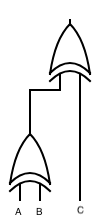
\includegraphics{circuits/3_input_xor.png}
%    \caption{3 input \XOR logic gate as cascading \XOR gates}
%    \label{f:my_label}
%    \ra{cf. new figure \ref{f:logical-subtractor01}}
%\end{figure}

\hh{
The first 2-\XOR (A and B) use the above implementation 
(i.e.~with heterodimer HrpRS) to regulate the expression of pchB. 
%
The 3rd inducer C then triggers the expression of pchA.
%
Similarly, only when pchB and pchA are co-expressed, the dimer pchBA can trigger the synthesis of salicylic acid, which then regulates the activator NahR to activate the expression of repressor McbR \cite{Rey2005}.

}

\begin{figure}
    \centering
    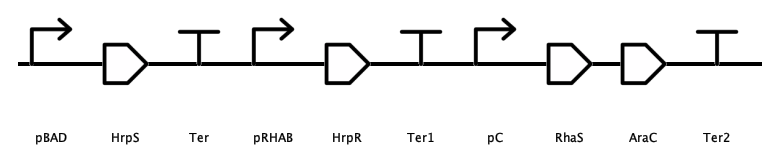
\includegraphics[width = \linewidth]{gene_circuits_xor/P1.png}
    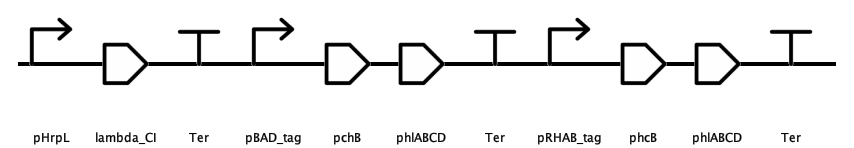
\includegraphics[width = \linewidth]{gene_circuits_xor/P2.png}
    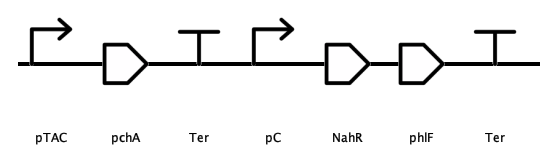
\includegraphics[width = \linewidth]{gene_circuits_xor/P3.png}
    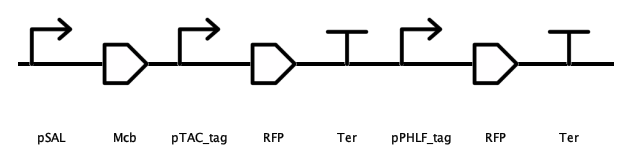
\includegraphics[width = \linewidth]{gene_circuits_xor/P4.png}
    \caption{Construct of layered \XOR gate. Inducer A, B and C are Ara, Rha and IPTG, which regulate the activity of pBAD, pRHAB and pTAC respectively. Here the tagged promoters refers to the ones that can be blocked by the upstream repressor. \hh{This is just a design sketch taht i came up with and drew with \url{https://sboldesigner.github.io}. For the final report we would use something looked nicer for the design diagram}
    \ra{if you keep them online please provide a url and/or upload all relevant files (not just the figures); also: vector graphics [delete when read]}
    }
    \label{f:gene_circuit_xor}
\end{figure}


\ra{Note: we don't do PNG b/c that doesn't scale well (neither up nor down). unfortunately, www.circuit-diagram.org doesn't export eps or pdf, but it does export svg, from which I make pdf [delete when read]}

%






\section{Simulations}

\subsection{PlayerA} \label{s:sim:player}

\url{https://github.com/numpde/ibiocomp/tree/main/code/20201231_SymBio_All/PlayerA}

\TODO{Some details missing}




%

\begin{figure}[hpbt]
	\begin{tabular}{cc|cc}
		\multicolumn{2}{c|}{\ce{\#r_1}} & \multicolumn{2}{c}{\ce{\#r_0}}
		%
		\\
		%
		\ce{\#w_A} = 0.1 & \ce{\#w_A} = 10 &
		\ce{\#w_A} = 0.1 & \ce{\#w_A} = 10 
		%
		\\
		%
		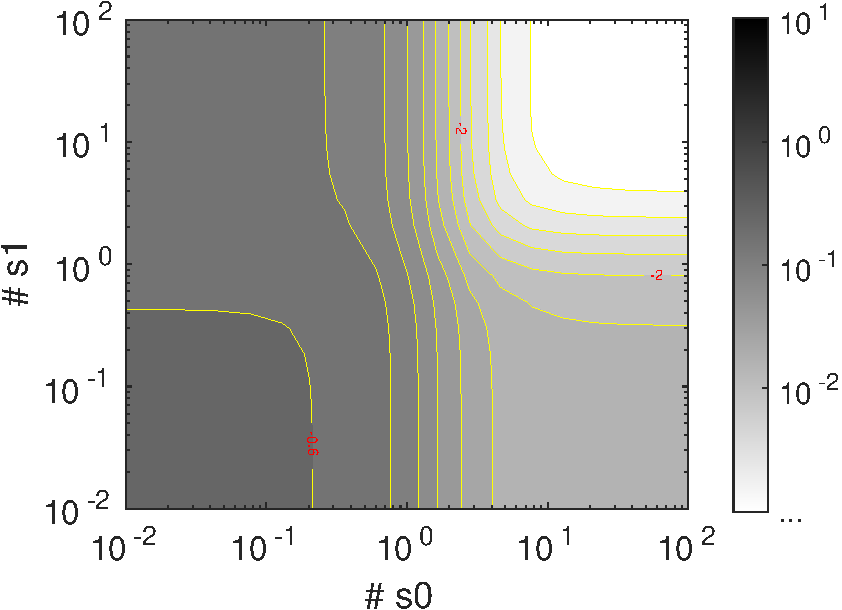
\includegraphics[width=0.22\textwidth]{PlayerA/response_r0__wA_in=0.1}
		&
		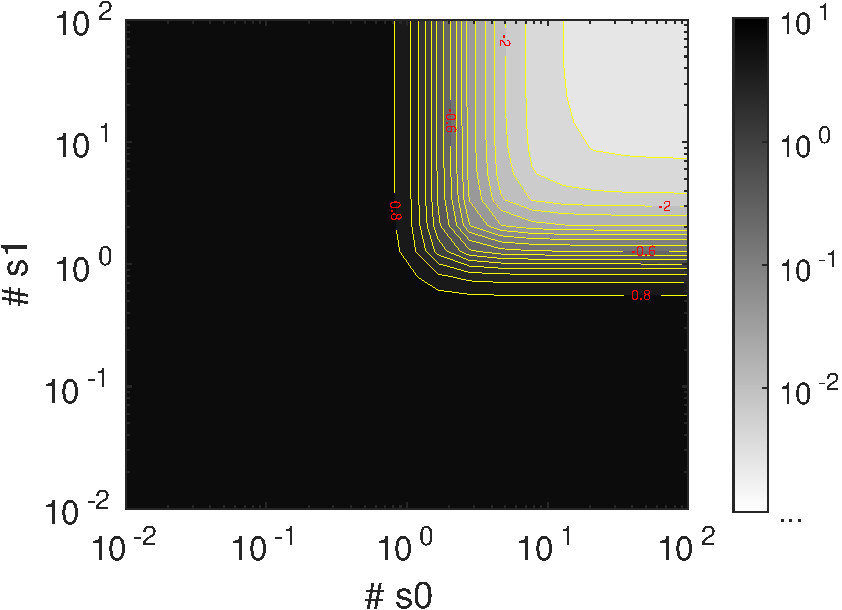
\includegraphics[width=0.22\textwidth]{PlayerA/response_r0__wA_in=10}
		&
		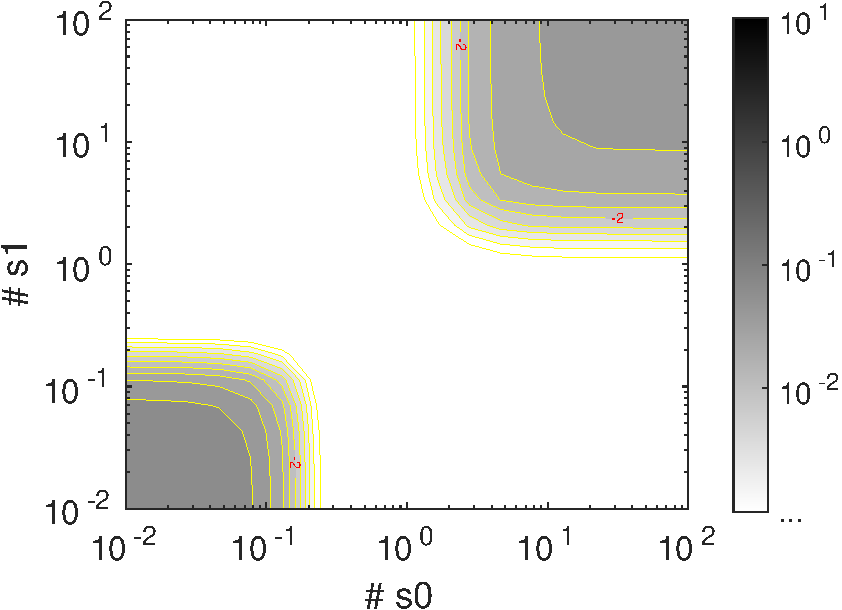
\includegraphics[width=0.22\textwidth]{PlayerA/response_r1__wA_in=0.1}
		&
		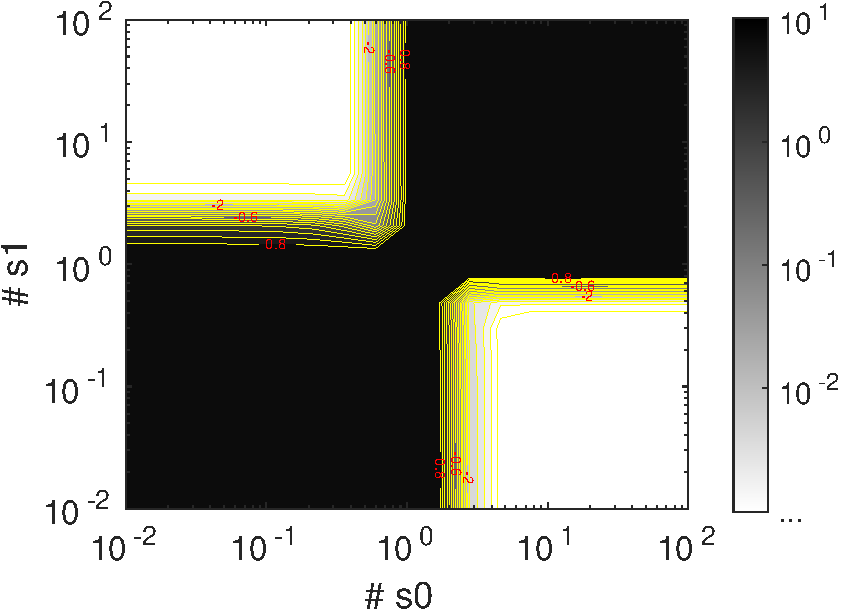
\includegraphics[width=0.22\textwidth]{PlayerA/response_r1__wA_in=10}
	\end{tabular}
	%
	\caption{%
		Response surfaces of Player A
		for varying \ce{\#s_1}($\uparrow$) and \ce{\#s_0}($\rightarrow$).
		%
		See \S\ref{s:sim:player}.
		%
		The log-colorbar goes from $10^{-3}$-or-less (white) to $10^1$ (black).
		%
		The yellow contour lines are at $10^t$, $t = 0.8, 0.6, 0.4, \ldots$.
	}
	%
	\label{f:player_response}
\end{figure}





\subsection{Bits 0, 2, 3}

Bits 0, 2, 3 are half-subtractors
which are technically a subfunctionality of Bit~1
(see Table~\ref{t:subtractor1}).
%
We omit closer discussion to focus on Bit~1.


\subsection{Bit 1} \label{s:sim:bit1}

\url{https://github.com/numpde/ibiocomp/tree/main/code/20201231_SymBio_All/Bit1}

\subsubsection*{c2} \label{s:sim:bit1:c2}



\subsubsection*{d1} \label{s:sim:bit1:d1}

Consider bit 1 of Subtractor A.
%
Suppose \ce{s_1 r_1 c_1 = 101},
in which case \ce{c_2 = 0}.
%
Suppose a transcription factor \ce{Y}
encoding \ce{c_2},
promotes expression of \ce{Xis} in the memory subunit.
%
%
When \ce{w_B} is up,
access to memory is on.
%
Since we want \ce{c_2 = 0},
the amount of \ce{Y} is low,
but
around the timepoint when 
\ce{w_B} is turned off
and the inputs begin to change,
\ce{Y} can experience a transient bump.
%
This is sufficient to produce \ce{Xis}
and thus to cause an unintended \emph{reset}
towards \ce{c_2 = 1}.
%
We found two ways to mitigate this
in the computational model.
%
One is to condition the expression of \ce{Xis}
on \ce{w_B} also
--
but this requires \ce{w_B} to go down
before other change
and could be sensitive to degradation rates.
%
A more robust way
is a buffer for \ce{Y}
(a ``shelf'')
that 
%
i)
has high affinity for \ce{Y};
%
ii)
sequesters 
a large amount of \ce{Y}
(about 30$\times$\href{https://en.wikipedia.org/wiki/EC50}{EC50} of $\ce{Y} \act \ce{Xis}$);
%
iii)
releases \ce{Y} for degradation when \ce{w_A} is on.
%
In this way, 
a transient increase in \ce{Y} is shelved
but a sustained signal 
(while \ce{w_B} is up)
will overflow the shelves and activate 
transcription of \ce{Xis}.
%
%
This is illustrated in Fig.~\ref{f:symbio-d1-tempo}.

\TODO{\ra{Issue: how to implement this ``Shelf''?}}
\ra{%
Note: This seems similar to
\cite[\href{{https://www.pnas.org/content/pnas/104/8/2643/F1.large.jpg?width=800&height=600&carousel=1}}{Fig.~1}]{WeberETAL2007},
also
\cite{NilgiriwalaETAL2014}.
}

%

\begin{figure}[hpbt]
	\begin{tabular}{cc|cc}
		\multicolumn{2}{c|}{\ce{\#d_1}} & \multicolumn{2}{c}{\ce{\#c_2}}
		%
		\\
		%
		\ce{\#c_1} = 0.1 & \ce{\#c_1} = 10 &
		\ce{\#c_1} = 0.1 & \ce{\#c_1} = 10 
		%
		\\
		%
		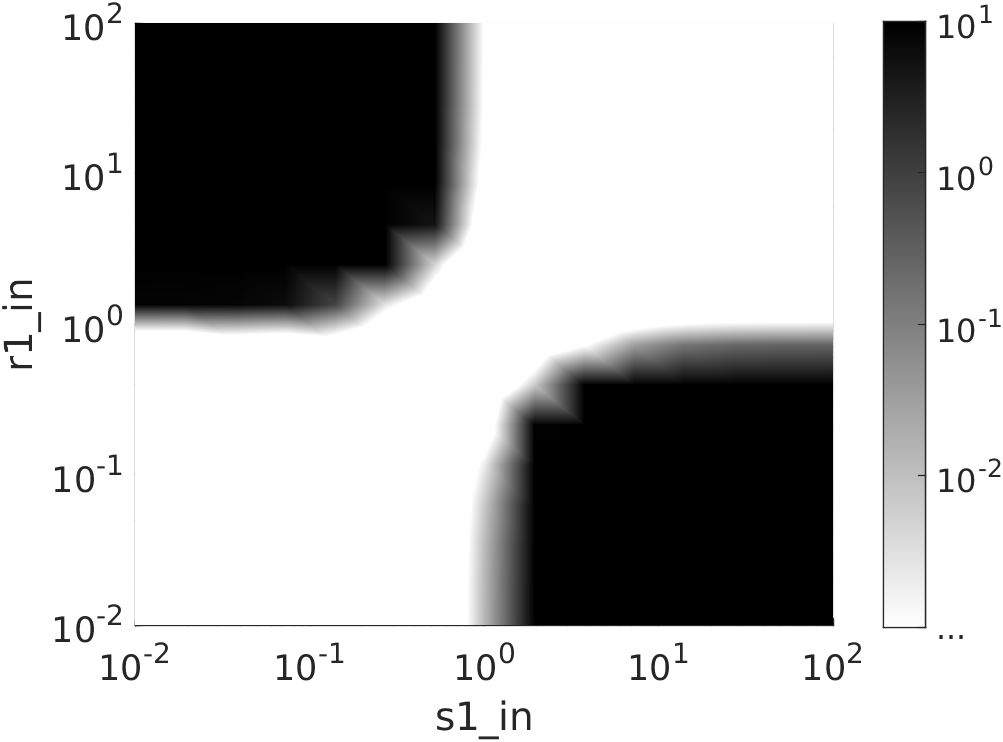
\includegraphics[width=0.22\textwidth]{Bit1/response_d1_final__c1_in=0.1}
		&
		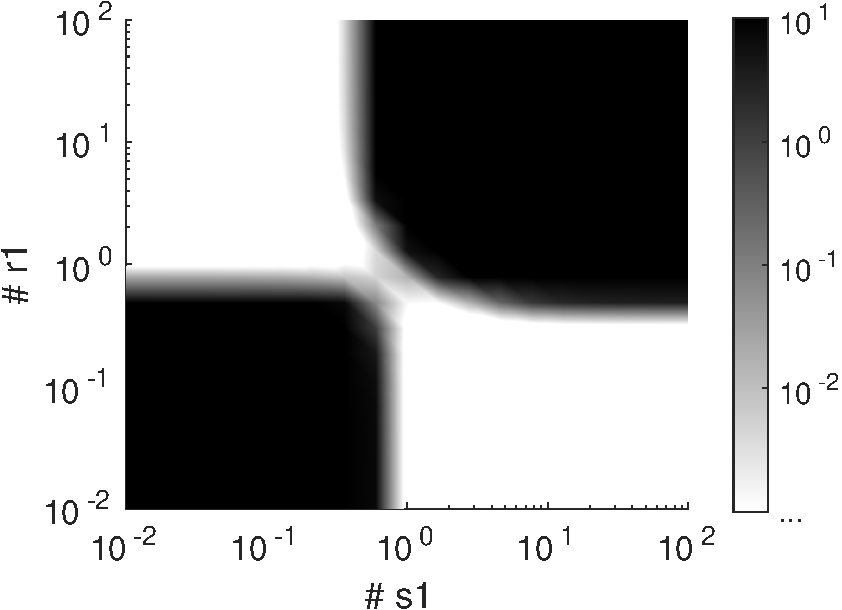
\includegraphics[width=0.22\textwidth]{Bit1/response_d1_final__c1_in=10}
		&
		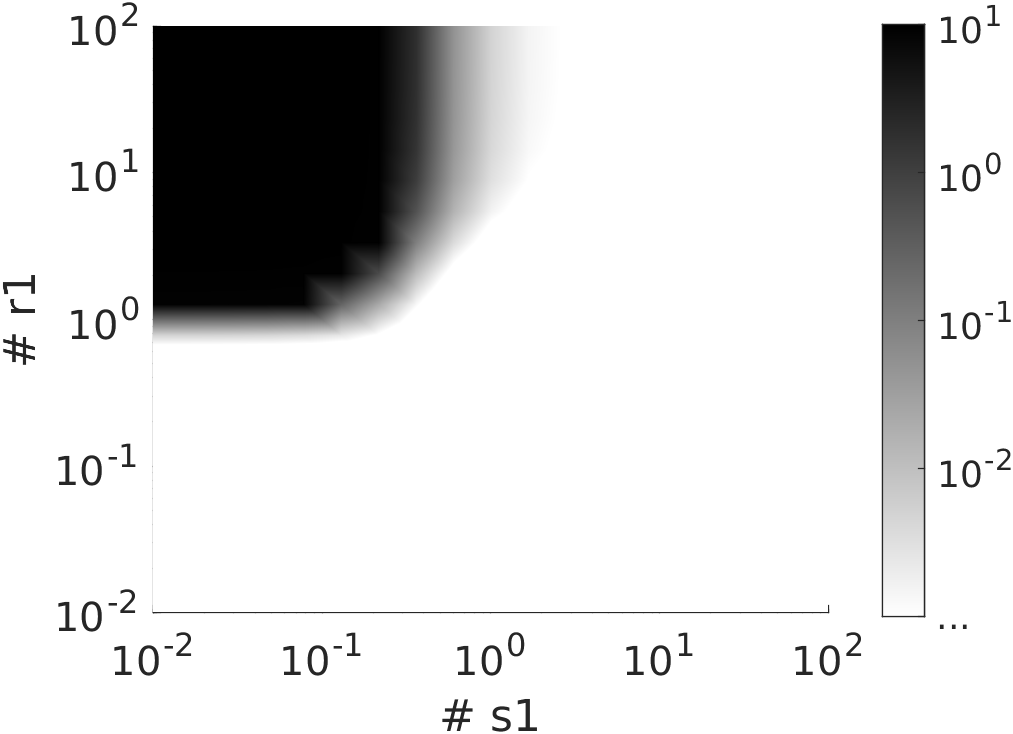
\includegraphics[width=0.22\textwidth]{Bit1/response_c2__c1_in=0.1}
		&
		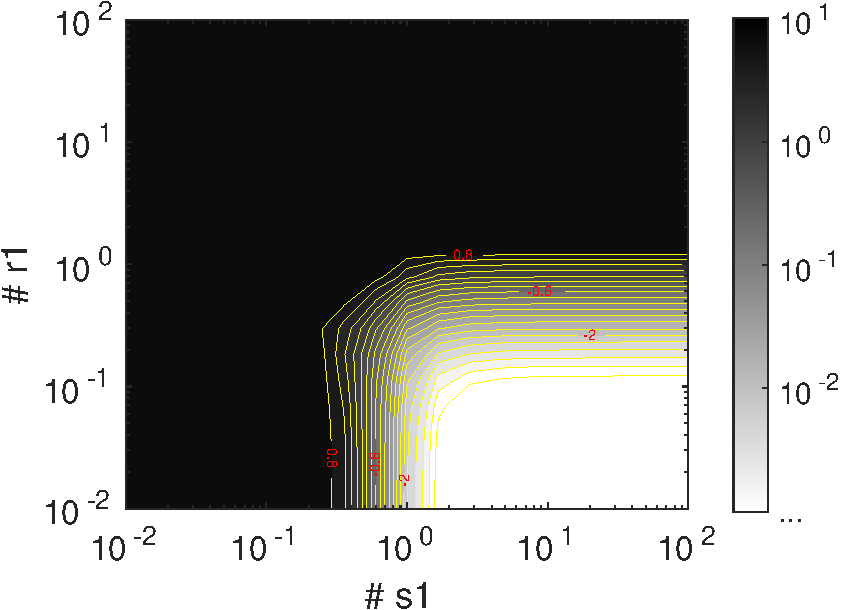
\includegraphics[width=0.22\textwidth]{Bit1/response_c2__c1_in=10}
	\end{tabular}
	%
	\caption{%
		Response surfaces of Subtractor A
		for varying \ce{\#r_1}($\uparrow$) and \ce{\#s_1}($\rightarrow$).
		%
		See \S\ref{s:sim:bit1}.
		%
		The output \ce{\#d_1}
		is measured after a compute-, inter- and readout-phase,
		cf.~Fig.~\ref{f:symbio-d1-tempo}.
		%
		The log-colorbar goes from $10^{-3}$-or-less (white) to $10^1$ (black).
		%
		The yellow contour lines are at $10^t$, $t = 0.8, 0.6, 0.4, \ldots$.
	}
	%
	\label{f:sub_response}
\end{figure}

%

\begin{figure}[phbt]
    \centering
    %
    \begin{overpic}[width=0.99\textwidth]{Bit1/response_d1_tempo}
    \put (50, 30) {%
    	\scalebox{0.7}{%
    		\begin{tabular}{c|ccc|c}
    		    & \ce{\#s_1} & \ce{\#r_1} & \ce{\#c_1} & $\approx \ce{\#d_1}$
    		    \\
    		    \hline
    		    \ce{B_1} & 10 & 10 & 10 & 0 
    		    \\
    		    \ce{A_1} & {\color{gray}$0.01$} & {\color{gray}$0.01$} & {\color{gray}$0.01$} & 10 
    		    \\
    		    \ce{B_2} & 10 & 10 & {\color{gray}$0.01$} & 0 
    		    \\
    		    \ce{A_2} & {\color{gray}$0.01$} & {\color{gray}$0.01$} & {\color{gray}$0.01$} & 0
    		    \\
    		\end{tabular}
    	}
    }
    \end{overpic}
    %
    \caption{%
        Subtractor A, bit 1, output \ce{\#d_1}
        across phases \ce{B_1}-\ce{A_1}-\ce{B_2}-\ce{A_2}
        (with interphases).
        %
        The table shows the inputs for each phase.
        %
        As required,
        we have
        $\#\ce{d_1} \approx 10$ 
        during the recall phase \ce{A_1}
        and
        $\#\ce{d_1} \approx 0$ 
        during the recall phase \ce{A_2}.
        %
        Observe the slight delay in the rise of Y
        at the beginning of \ce{B_1} while it is being ``shelved''
        and a sustained supply by ``unshelving'' at the end
        that helps maintaining Xis;
        conversely,
        the leakage of Y is ``shelved''
        during \ce{B_2}
        preventing unwanted expression of Xis.
        %
        See also \S\ref{s:sim:bit1:d1}/p.\pageref{s:sim:bit1:d1}.
    }
    %
    \label{f:symbio-d1-tempo}
\end{figure}

%

\section{Discussion}

\TODO{risks}



\section{Acknowledgments}

\TODO{ack}




\footnotesize
\bibliographystyle{apalike}
\bibliography{refs}
\normalsize

\clearpage


\section*{Appendix}

\subsection{Subtractor module}

Fig.~\ref{f:logical-subtractor01} 
shows the main principles
behind 
the Subtractor module (bit 0 and bit 1),
but our implementation
differs in the details.
%
In particular, we use a reversible recombinase
for the memory module, see \S\ref{ss:memory}/p.\pageref{ss:memory}.

% https://www.circuit-diagram.org/editor/c/075f8cf9d084400b94f1384cc1c3ba96
\begin{figure}[phbt]
\centering
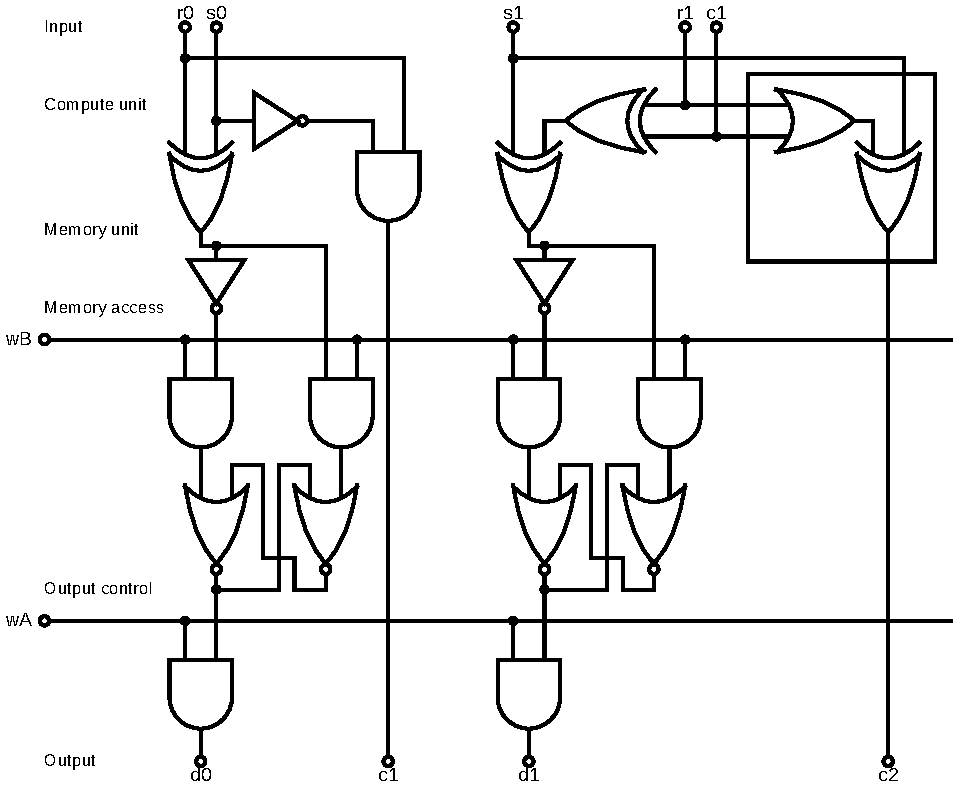
\includegraphics[width=0.9\linewidth]{circuits/Logical-HalfSubtractor0.svg.pdf}
%
\caption{%
Bit~0 and Bit~1
of
Subtractor~A.
%
The result of the compute unit is written to the memory unit
(e.g.~a bistable switch)
when the signal \ce{w_B} is present.
%
The value of the memory unit is
forwarded to the output
when the signal \ce{w_A} is present.
}
\label{f:logical-subtractor01}
\end{figure}




\subsection{Cross-inhibition \texorpdfstring{\AND}{AND} gate} \label{s:x-inh}

\TODO{explain}

\ra{
this is implemented in \ce{c_2}
[\href{https://i.ibb.co/86S2qfL/2021-01-17-01-42-06.png}{fig}]
}


\subsection{Kinetics}

\TODO{explain guidelines}

\subsubsection*{AmtR}

We assume
the mechanism
\begin{subequations}
\[
	\ce{
		2 \protein{AmtR} + \promoter{AmtR}
		& <=>>
		\protein{AmtR}_2 \with \promoter{AmtR}
	}
	%
	\\
	%
	\ce{
		\promoter{AmtR} 
		& ->
		\promoter{AmtR} + \protein{Output}
	}
\]
\end{subequations}
and
the kinetics:
\begin{subequations}
\[
	\label{e:AmtR_Act}
	%
	\promoter{AmtR} 
	& =
	\frac{1}{1 + k_{\ref{e:AmtR_Act}} \protein{AmtR}^{n_{\ref{e:AmtR_Act}}}}
	\promoter{AmtR}_\text{total}
	%
	% here, k = forward / backward
	%
	,
	\\
	%
	\label{e:AmtR_Out}
	%
	\tfrac{\d}{\d{t}}
	\protein{Output} 
	& =
	k_{\ref{e:AmtR_Out}}
	\promoter{AmtR}
	.
\]
\end{subequations}


\subsubsection*{3OC6}


We write
$\protein{LuxR^\star}$ for $\signal{3OC6\text{-}HSL} \with \protein{LuxR}$
and
$\promoter{Lux^\star}$ for $\protein{LuxR^\star} \with \promoter{Lux}$.
%
%\TODO{
%Let $\protein{LuxR^\star}$ denote 
%the activated form
%$\signal{3OC6}:\protein{LuxR}$.
%}
%
%
We assume the mechanism:
%
\begin{subequations}
\[
	\ce{
		\signal{{3OC6}} + \protein{LuxR}
		& <=>>
		\protein{LuxR^\star}
	}
	\\
	\ce{
		\protein{LuxR^\star} + \promoter{Lux}
		& <=>>
		\promoter{Lux^\star}
	}
	\\
	\ce{
		\promoter{Lux^\star}
		& ->
		\promoter{Lux^\star} + \protein{Output}
	}
	.
\]
\end{subequations}
%
%=======
%	\protein{LuxR^\star} + \protein{RNApol} + \promoter{P_{Lux}}
%	& \longleftrightarrow
%	\protein{LuxR^\star} + \protein{RNApol} : \promoter{P_{Lux}}
%	\\
%	\protein{RNApol} : \promoter{P_{Lux}}
%	& \longrightarrow
%	\protein{RNApol} + \promoter{P_{Lux}} + \protein{Output}
%>>>>>>> c8a0f57bdb0a7b80747263819cbb64562e087765
%\TODO{
%\[
%	\signal{3OC6} + \protein{LuxR}
%	& \longleftrightarrow
%	\protein{LuxR^\star}
%	\\
%	\protein{LuxR^\star} + \protein{RNApol} + \promoter{Lux}
%	& \longleftrightarrow
%	\protein{LuxR^\star} + \protein{RNApol} : \promoter{Lux}
%	\\
%	\protein{RNApol} : \promoter{Lux}
%	& \longrightarrow
%	\protein{RNApol} + \promoter{Lux} + \protein{Output}
%\]
%}
% https://chem.libretexts.org/Bookshelves/Biological_Chemistry/Supplemental_Modules_(Biological_Chemistry)/Enzymes/Enzymatic_Kinetics/Sigmoid_Kinetics
%
%
%
and the kinetics:
%
\begin{subequations}
\[
	\label{e:LuxR_Act}
	%
	\protein{LuxR^\star} 
	& =
	\frac{
		\signal{{3OC6}}
	}{
		k_{\ref{e:LuxR_Act}} + \signal{{3OC6}}
	}
	\protein{LuxR}_\text{total}
%	\TEXT{initially}
%	\protein{LuxR^\star} = 0
	,
	%
	\\
	%%
	\label{e:P_Lux_Act}
	%
	\promoter{Lux^\star} 
	& =
	\frac{
		\protein{LuxR^\star}
	}{
		k_{\ref{e:P_Lux_Act}} + \protein{LuxR^\star}
	}
	\promoter{Lux}_\text{total}
%	\TEXT{initially}
%	\promoter{Lux^\star} = 0
	,
	%
	\\
	%
	\label{e:P_Lux_Out}
	%
	\tfrac{\d}{\d{t}}
	\protein{Output}
	& =
	k_{\ref{e:P_Lux_Out}} \promoter{Lux^\star}
	.
\]
\end{subequations}
%
%
In combination, we have
\[
	\tfrac{\d}{\d{t}}
	\protein{Output}
	=
	k_{\ref{e:P_Lux_Out}}
	\promoter{Lux}_\text{total}
	\frac{
		\signal{} \protein{}_\text{total}
	}{
		k_{\ref{e:LuxR_Act}} k_{\ref{e:P_Lux_Act}}
		+
		k_{\ref{e:P_Lux_Act}} \signal{}
		+
		\signal{} \protein{}_\text{total}
	}
	.
\]


\subsubsection*{Sal}


We write
$
	\promoter{Sal^\star} :=
	\signal{Sal}_4 \with \protein{NahR}_4 \with \promoter{Sal}
$
for the active form.
%
%
We assume the mechanism
%
\begin{subequations}
\[
	\ce{
		\signal{Sal} + 
		\signal{Sal}_{k - 1} \with \protein{NahR}_4 \with \promoter{Sal}
		& <=>>
		\signal{Sal}_k \with \protein{NahR}_4 \with \promoter{Sal}
	}
	,
	\quad \text{k} = 1, 2, 3, 4,
	%
	%
	\\
	%
	%
	\ce{
		\promoter{Sal^\star}
		&
		->
		\promoter{Sal^\star} + \protein{Output}
	}
\]
\end{subequations}
%
%Mechanism (here \protein{NahR^\star} denotes the activated (tetramer) form):
%\[
%	\signal{Sal} + \protein{NahR}
%	& \longleftrightarrow
%	\protein{NahR^\star}
%	 \\
%	 \protein{NahR^\star} + \protein{RNApol} + \promoter{P_{Sal}}
%	& \longleftrightarrow
%	\protein{NahR^\star} + \protein{RNApol} : \promoter{P_{Sal}}
%	\\
%	\protein{RNApol} : \promoter{P_{Sal}}
%	& \longrightarrow
%	\protein{RNApol} + \promoter{P_{Sal}} + \protein{Output}
%	.
%\]
%
%
which we implement as:
%
\begin{subequations}
\[
	\label{e:NahR_Act}
	%
	\promoter{Sal^\star}
	& =
	\frac{
		\signal{}^{n_{\ref{e:NahR_Act}}}
	}{
		k_{\ref{e:NahR_Act}} + \signal{}^{n_{\ref{e:NahR_Act}}}
	}
	\promoter{Sal}_\text{total}
	,
	%
	%
	\\
	%
	%
	\label{e:NahR_Out}
	%
	\tfrac{\d}{\d{t}}
	\protein{Output}
	& =
	k_{\ref{e:NahR_Out}} 
	\promoter{Sal^\star}
	.
\]
\end{subequations}






\clearpage

\section*{Final TODOs}

\TODO{spacing of act and rep}

\TODO{check that Table \ref{t:signals} is correct}


\clearpage

\SHOWTODOS




\leavevmode\vfill{\tiny\color{lightgray}\hfill{\DTMnow}}
\end{document}





